\chapter{METODOLOGI}

Penelitian ini dilaksanakan sesuai dengan blok diagram pada Gambar 3.1. Blok diagram tersebut
merupakan metodologi penelitian yang disusun sesuai dengan langkah-langkah yang dilakukan dalam penelitian ini.

\begin{figure} [ht] \centering
  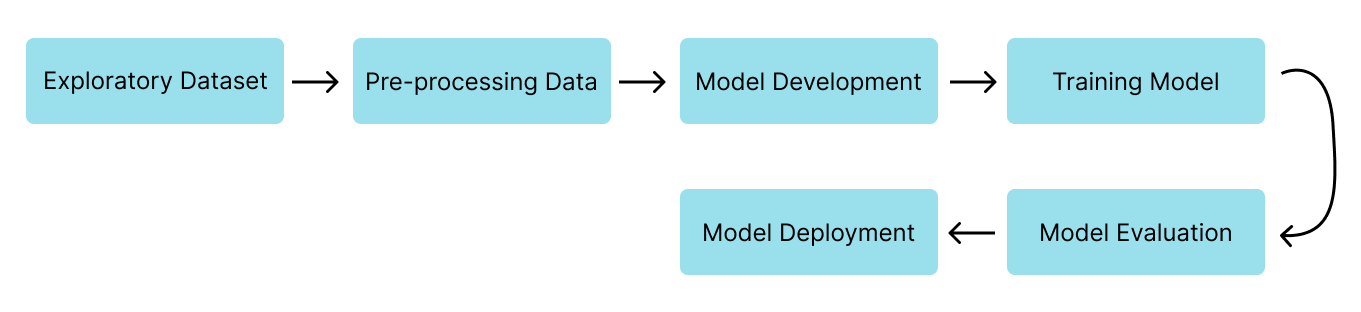
\includegraphics[width=160mm]{gambar/diagram-blok.png}
  \caption{Metodologi Penelitian}
\end{figure}


\section{Exploratory Dataset}
Melakukan analisa pada data untuk mendapatkan gambaran awal pada data. Analisa yang dilakukan yaitu
memeriksa informasi pada data (tipe data pada tiap data), memeriksa \emph{missing value} {(data yang hilang pada baris data)},
memeriksa duplikasi pada data.


\section{Pre-processing Data}
Pada proses ini dataset yang telah dilakukan analisa akan dilakukan pra-pemrosesan sebelum dataset dapat digunakan
untuk melakukan pelatihan pada model. Pada sistem rekomendasi pra-pemrosesan data yang biasa dilakukan seperti menghapus data
yang tidak diperlukan untuk proses pelatihan, menghapus \emph{missing value} jika ada, melakukan normalisasi pada data (biasanya mentransformasikan data kedalam range yang sama),
melakukan pembagian data pelatihan dan data percobaan.

\section{Model Development}
Pembuatan model menggunakan dua pendekatan yaitu \emph{content-based filtering} dan \emph{collaborative filtering} dengan menggunakan metode \emph{Deep Learning}. Teknik
\emph{content-based filtering} akan merekomendasikan mata kuliah yang benar benar mirip dengan mata kuliah yang pernah dipilih oleh mahasiswa sebelumnya. Sedangkan, \emph{collaborative filtering}
memerlukan parameter pembanding yang akan digunakan untuk dipelajari oleh model nantinya. Pada kasus ini parameter pembanding yang akan digunakan yaitu nilai mata kuliah mahasiswa.

\section{Training Model}
Melakukan pelatihan pada dataset menggunakan yang telah dibuat sebelumnya untuk menemukan pola pada data dan dapat memberikan rekomendasi yang baik kepada mahasiswa.

\section{Model Evaluation}
Evaluasi Model dilakukan dengan melakukan rekomendasi pada data percobaan. Jika dirasa rekomendasi belum cukup baik. Maka perlu melakukan
\emph{tuning parameter} pada model seperti unit layer, jumlah layer pada model \emph{Deep Learning}, jumlah iterasi pelatihan dan beberapa parameter lain hingga model dapat memberikan rekomendasi dengan cukup baik.

\section{Model Deployment}
Pada tahap ini model dari sistem rekomendasi yang telah dibuat sebelumnya ada dideploy atau dirilis agar dapat digunakan untuk memberikan rekomendasi melalui sebuah \emph{software}.
\emph{Software} yang digunakan untuk menampilkan rekomendasi dari mata kuliah yang diberikan oleh model tersebut berupa website sederhana yang bisa menampilkan daftar mata kuliah
yang direkomendasikan sesuai dengan ID/NRP dari mahasiswa.

\begin{figure} [ht] \centering
  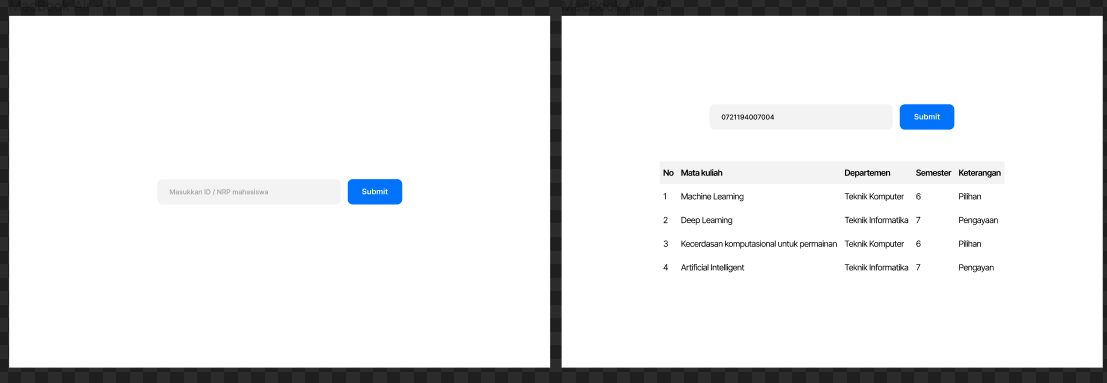
\includegraphics[width=160mm]{gambar/mockup.png}
  \caption{Mock Up Tampilan Website Sederhana}
\end{figure}

